\documentclass[utf8]{ctexart}

\usepackage[a4paper,left=1.25in,right=1.25in,top=1in,bottom=1in]{geometry}
\usepackage{listings}
\usepackage{graphicx}
\usepackage{caption}
\usepackage{subfigure}
\usepackage{booktabs}
\usepackage{amsmath}
\usepackage{amsthm}
\usepackage{amsfonts}
\usepackage{float}
\usepackage{indentfirst}
\usepackage{tikz}
\usetikzlibrary{shapes,arrows}
\usetikzlibrary{shapes.geometric, arrows}
\usepackage{algorithm}
\usepackage{algorithmic}
\usepackage{newclude}
\usepackage[perpage]{footmisc}

\graphicspath{ {images/} }
\raggedbottom	% 令页面在垂直方向向顶部对齐
\renewcommand\qedsymbol{QED}
\newcommand{\sign}[1]{\mathrm{sgn}(#1)}
\everymath{\displaystyle}   % 行内公式采用行间公式格式排列
\pagestyle{plain}

\title{《计算机辅助几何设计》第六次作业}
\author{姓名:殷文良\qquad 学号:12435063}
\date{\today}

\begin{document}
\maketitle
\ctexset { section = { format={\Large \bfseries } } }

\section*{思考题 1}
\subsection*{1.}
\begin{proof}
    双曲线$x^2-y^2=1$的有理参数形式为
    $$
    \begin{cases}
    x(u) &= \frac{1+u^2}{1-u^2},\\
    y(u) &= \frac{2u}{1-u^2},
    \end{cases}\quad
    -\infty < u < \infty, u\ne \pm 1.
    $$
    由端点插值性和端点相切性可知,$P_0=(1,0),P_1=(1,\sqrt{2}-1),P_2=(\sqrt{2},1)$。根据
    $W(u)=1-u^2=\sum_{i=0}^2B_{i,2}(u)\omega_i = (1-u)^2\omega_0 + 2u(1-u)\omega_1+u^2\omega_2$。令
    $u=0$,得$\omega_0=1$;令$u=1$,得$\omega_2 = 0$;令$u=\frac{1}{2}$,得$\frac{3}{4}=\frac{1}{4}\omega_0 + \frac{1}{2}\omega_1+\frac{1}{4}\omega_2$,由
    $\omega_0=1,\omega_2=0$,得$\omega_1 = 1$。于是,双曲线的2次有理Bezier曲线表示为
    $$
    C(u) = \frac{(1-u)^2P_0 + 2u(1-u)P_1}{(1-u)^2 + 2u(1-u)}.
    $$
\end{proof}
\subsection*{2.}
\begin{proof}
    只证明椭圆情形,双曲线同理可证。\\
    不失一般性,我们证明$xy$平面上中心在原点的椭圆不能用整曲线表示。采用反证法,不妨设
    $$
    x(u) = a_0+a_1u+\cdots + a_nu^n\quad y(u) = b_0+b_1u+\cdots+b_nu^n
    $$
    由于$\frac{x^2}{a^2}+\frac{y^2}{b^2}=1$,因此有
    $$
    \begin{aligned}
    0 &= \frac{1}{a^2}(a_0+a_1u+\cdots+a_nu^n)^2 + \frac{1}{b^2}(b_0+b_1u+\cdots + b_nu^n)^2 - 1\\
    &= (\frac{a_0^2}{a^2}+\frac{b_0^2}{b^2}-1) + 2(\frac{a_0a_1}{a^2}+\frac{b_0b_n}{b^2})u + (\frac{a_1^2}{a^2}+2\frac{a_0a_2}{a^2}+\frac{b_1^2}{b^2}+2\frac{b_0b_2}{b^2})u^2\\
    &\quad + \cdots + (\frac{a_{n-1}^2}{a^2}+2\frac{a_{n-2}a_n}{a^2}+\frac{b_{n-1}^2}{b^2}+2\frac{b_{n-2}b_n}{b^2})u^{n-2}\\
    &\quad + 2(\frac{a_na_{n-1}}{a^2}+\frac{b_nb_{n-1}}{b^2})u^{2n-1} + (\frac{a_n^2}{a^2}+\frac{b_n^2}{b^2})u^{2n}
    \end{aligned}
    $$
    上式应对所有$u$都成立,即上式右端所有项的系数都为0,。从最高次开始推导,由高到低,经过$n$步我们可以证明对所有的$i=1,2,\cdots,n$,
    有:$a_i=0,b_i=0$。最后,我们得到$x(u)=a_0,y(u)=b_0$,显然它不是一个椭圆,这和假设矛盾。
\end{proof}

\subsection*{3.}
\begin{proof}
    考虑圆心在原点,半径为$r$的半圆(见图\ref{fig: half_circ})。令$P_0^{\omega}=(r,0,1),P_1^{\omega}=(0,r,0),P_2^{\omega}=(-r,0,1)$。

    \begin{figure}[H]
        \centering
        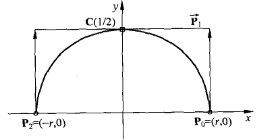
\includegraphics[width=0.5\textwidth]{half_circ.png}
        \caption{使用无穷远点来定义半圆}
        \label{fig: half_circ}
    \end{figure}
    对半圆进行升阶可得
    $$
    \begin{aligned}
        &Q_0^{\omega} = P_0^{\omega},\quad Q_3^{\omega} = P_2^{\omega}\\
        &Q_1^{\omega} = \frac{1}{3}P_0^{\omega} + \frac{2}{3}P_1^{\omega} = (\frac{1}{3}r, \frac{2}{3}r,\frac{1}{3}r)\\
        &Q_2^{\omega} = \frac{2}{3}P_1^{\omega} + \frac{1}{3}P_2^{\omega} = (-\frac{1}{3}r, \frac{2}{3}r,\frac{1}{3}r)
    \end{aligned}
    $$
    因此(见图\ref{fig: half_circ2})
    $$
    \begin{aligned}
        \{\omega_i\} &= \{1,\frac{1}{3},\frac{1}{3},1\},\\
        \{Q_i\} &= {(r,0),(r,2r),(-r,2r),(-r,0)}.
    \end{aligned}
    $$
    \begin{figure}[H]
        \centering
        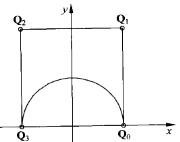
\includegraphics[width=0.5\textwidth]{half_circ2.png}
        \caption{半圆的三次有理Bezier表示}
        \label{fig: half_circ2}
    \end{figure}

\end{proof}

\end{document}
